%%%%%%%%%%%%%%%%%%%%%%%%%%%%%%%%%%%%%%%%%%%%%%%%%%%%%%%%%%%%%%%%%%%%%%
% How to use writeLaTeX: 
%
% You edit the source code here on the left, and the preview on the
% right shows you the result within a few seconds.
%
% Bookmark this page and share the URL with your co-authors. They can
% edit at the same time!
%
% You can upload figures, bibliographies, custom classes and
% styles using the files menu.
%
%%%%%%%%%%%%%%%%%%%%%%%%%%%%%%%%%%%%%%%%%%%%%%%%%%%%%%%%%%%%%%%%%%%%%%

\documentclass[12pt]{article}

\usepackage{sbc-template}

\usepackage{graphicx,url}

\usepackage[brazil]{babel}   
\usepackage[utf8]{inputenc}  

\usepackage{fancyhdr}
\pagestyle{fancy}

\fancyhead[L]{ }
\fancyhead[R]{ }

%\chead{\begin{picture}(3,3) \put(-230,-15) {\includegraphics%[width=16cm, height=2.8cm, keepaspectratio=false]{logoSIRC.png}} \end{picture}}
\renewcommand{\headrulewidth}{0pt}
\sloppy
\begin{document} 


\title{Relatório Técnico Sobre o Avanço Pandemia Causada pelo Vírus SARS-CoV-2 na Cidade de Dourados, MS\\ Análise de Dados, Comparações de Cenários e Modelo Preditivo}

\author{Fernando Ferraz Ribeiro\inst{1}, Rafael H. Bordini\inst{2}, Flávio Rech
  Wagner\inst{1}, Jomi F. Hübner\inst{3} }
  


\address{Universidade Federal da Bahia -- Faculdade de Arquitetura -- LCAD
  (UFBA)\\
  Salvador, BA -- Brasil
\nextinstitute
  Department of Computer Science -- University of Durham\\
  Durham, U.K.
\nextinstitute
  Departamento de Sistemas e Computação\\
  Universidade Regional de Blumenal (FURB) -- Blumenau, SC -- Brazil
  \email{fernando.ribeiro@ufba.br, R.Bordini@durham.ac.uk,
  jomi@inf.furb.br}
}


\maketitle

\begin{abstract}
  This report presents a study on the progress of the pandemic caused by the Sars-Cov2 virus in the municipality of Dourados, MS. For this purpose, the database provided by the Ministry of Health was used. The report presents a descriptive analysis of the data available in that database. A comparison with the cases diagnosed in other municipalities in the same state and with data from the city of Manaus, AM, used as a reference for an emblematic case of the advance of the pandemic in Brazil. In the end, a predictive model adapted from DELPHI, developed by a research team linked to MIT, used as an instrument to visualize the future scenario where current trends of progress are maintained and confirmed.
\end{abstract}
     
\begin{resumo} 
  Este relatório apresenta um estudo sobre o avanço da pandemia causada pelo vírus Sars-Cov2 no município de Dourados, MS. Para tanto foi utilizada a base de dados fornecida pelo Ministério da Saúde. O relatório apresenta uma análise descritiva dos dados disponíveis na referida base. Uma comparação com os casos diagnosticados em outros municípios do mesmo estado e com os dados da cidade de Manaus, AM, utilizado como referência de um caso emblemático do avanço da pandemia no Brasil. Ao fim, um modelo preditivo adaptado do DELPHI, desenvolvido pro uma equipe de pesquisa vinculada ao MIT, utilizado como instrumento de visualização do cenário futuro onde as atuais tendências de avanço sejam mantidas e confirmadas.
\end{resumo}


\section{Introdução}

O avanço da pandemia da covid-19, causada pelo vírus SARS-CoV-2, tem se apresentado como o mais importante desafio do tempo presente. Autoridades políticas, cientistas e a sociedade tem buscado se organizar com o intuito de minimizar os grandes malefícios, direta ou indiretamente ligados à propagação desta enfermidade. De acordo com a \textit{Johns Hopkins University}, uma das principais fontes de dados mundiais sobre o tema, o número de casos confirmados no mundo já ultrapassa os 9 milhões (em 23/06/2020).

A adequada coleta e análise dos dados relativos à pandemia tem sido uma importante ferramenta no enfrentamento desta crise, sendo usada para direcionar ações, recursos e informações em todas as esferas da sociedade, na procura de um caminho menos calamitoso na lida com este nebuloso cenário.

No presente trabalho, uma análise dos dados da cidade de Dourados, MS e apresentada. A situação da cidade é comparada com os demais municípios do estado e a curva de crescimento registrada na referida cidade é comparada com a curva registrada na cidade de Manaus, AM. Em seguida os dados são utilizados para alimentar um modelo preditivo baseado no DELPHI, desenvolvido por uma equipe de pesquisadores ligada ao MIT. Na conclusão, os resultados obtidos são analisados e possíveis desdobramentos de pesquisa sugeridos. 

\section{First Page} \label{sec:firstpage}

The first page must display the paper title, the name and address of the
authors, the abstract in English and ``resumo'' in Portuguese (``resumos'' are
required only for papers written in Portuguese). The title must be centered
over the whole page, in 16 point boldface font and with 12 points of space
before itself. Author names must be centered in 12 point font, bold, all of
them disposed in the same line, separated by commas and with 12 points of
space after the title. Addresses must be centered in 12 point font, also with
12 points of space after the authors' names. E-mail addresses should be
written using font Courier New, 10 point nominal size, with 6 points of space
before and 6 points of space after.

The abstract and ``resumo'' (if is the case) must be in 12 point Times font,
indented 0.8cm on both sides. The word \textbf{Abstract} and \textbf{Resumo},
should be written in boldface and must precede the text.

\section{CD-ROMs and Printed Proceedings}

In some conferences, the papers are published on CD-ROM while only the
abstract is published in the printed Proceedings. In this case, authors are
invited to prepare two final versions of the paper. One, complete, to be
published on the CD and the other, containing only the first page, with
abstract and ``resumo'' (for papers in Portuguese).

\section{Sections and Paragraphs}

Section titles must be in boldface, 13pt, flush left. There should be an extra
12 pt of space before each title. Section numbering is optional. The first
paragraph of each section should not be indented, while the first lines of
subsequent paragraphs should be indented by 1.27 cm.

\subsection{Subsections}

The subsection titles must be in boldface, 12pt, flush left.

\section{Figures and Captions}\label{sec:figs}


Figure and table captions should be centered if less than one line
(Figure~\ref{fig:exampleFig1}), otherwise justified and indented by 0.8cm on
both margins, as shown in Figure~\ref{fig:exampleFig2}. The caption font must
be Helvetica, 10 point, boldface, with 6 points of space before and after each
caption.

\begin{figure}[!htb]
\centering
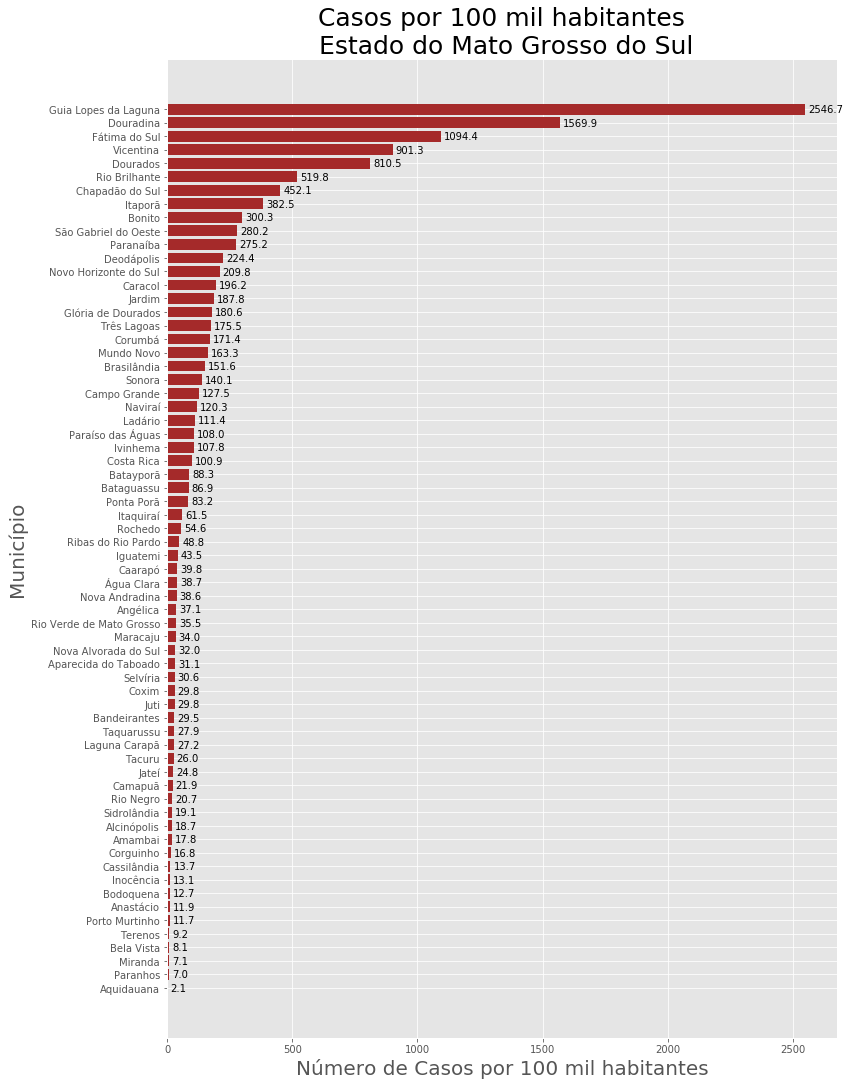
\includegraphics[width=1\textwidth]{figs/casos_100_mil_por_municipio.png}
\caption{Número de casos diagnosticados por município (MS)}
\label{fig:casosMuni100k}
\end{figure}

\begin{figure}[ht]
\centering
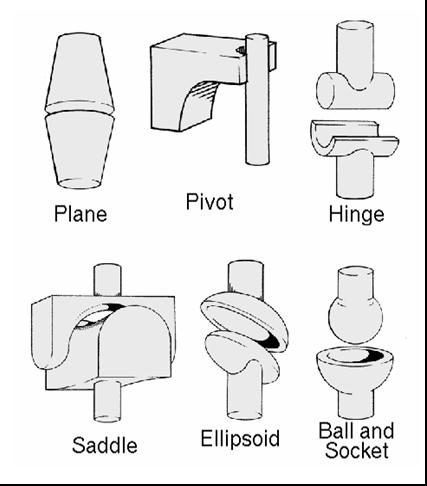
\includegraphics[width=.3\textwidth]{fig2.jpg}
\caption{This figure is an example of a figure caption taking more than one
  line and justified considering margins mentioned in Section~\ref{sec:figs}.}
\label{fig:exampleFig2}
\end{figure}

In tables, try to avoid the use of colored or shaded backgrounds, and avoid
thick, doubled, or unnecessary framing lines. When reporting empirical data,
do not use more decimal digits than warranted by their precision and
reproducibility. Table caption must be placed before the table (see Table 1)
and the font used must also be Helvetica, 10 point, boldface, with 6 points of
space before and after each caption.

\begin{table}[ht]
\centering
\caption{Variables to be considered on the evaluation of interaction
  techniques}
\label{tab:exTable1}
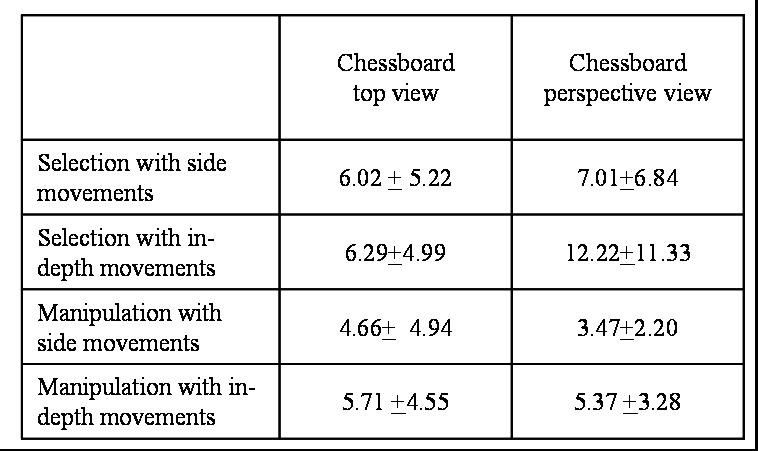
\includegraphics[width=.7\textwidth]{table.jpg}
\end{table}

\section{Images}

All images and illustrations should be in black-and-white, or gray tones,
excepting for the papers that will be electronically available (on CD-ROMs,
internet, etc.). The image resolution on paper should be about 600 dpi for
black-and-white images, and 150-300 dpi for grayscale images.  Do not include
images with excessive resolution, as they may take hours to print, without any
visible difference in the result. 

\section{References}

Bibliographic references must be unambiguous and uniform.  We recommend giving
the author names references in brackets, e.g. \cite{knuth:84},
\cite{boulic:91}, and \cite{smith:99}.

The references must be listed using 12 point font size, with 6 points of space
before each reference. The first line of each reference should not be
indented, while the subsequent should be indented by 0.5 cm.

\bibliographystyle{sbc}
\bibliography{sbc-template}

\end{document}
